\subsection*{Visual Representations of Relations}
In Progress Check~\ref{prog:setofpairs}, we were able to draw a graph of a relation as a way to visualize the relation.  In this case, the relation was a function from $\R$ to $\R$.  In addition, in Progress Check~\ref{A:relationexamples}, we were also able to use a graph to represent a relation.  In this case, the graph of the relation $T = \left\{ {\left( {x, y} \right) \in \mathbb{R} \times \mathbb{R}   \mid x^2  + y^2  = 64} \right\}$ is a circle of radius 8 whose center is at the origin.

When $R$ is a relation from a subset of the real numbers $\R$ to a subset of $\R$, we can often use a graph to provide a visual representation of the relation.  This is especially true if the relation is defined by an equation or even an inequality.  For example, if
\[
R = \left\{ (x, y) \in \R \times \R \mid y \geq x^2 \right\},
\]
then we can use the following graph as a way to visualize the points in the plane that are also in this relation.
\begin{figure}[h]
\begin{center}
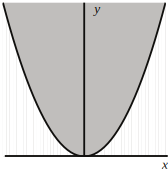
\includegraphics{figps-sec71-graph.eps}
\caption{Graph of $y \geq x^2$} \label{fig:graph-relation}
\end{center}
\end{figure}

\newpar
The points $(x, y)$ in the relation $R$ are the points on the graph of $y = x^2$ or are in the shaded region.  This because for these points, $y \geq x^2$. One of the shortcomings of this type of graph is that the graph of the equation and the shaded region are actually unbounded and so we can never show the entire graph of this relation.  However, it does allow us to see that the points in this relation are either on the parabola defined by the equation $y = x^2$ or are ``inside'' the parabola.

When the domain or range of a relation is infinite, we cannot provide a visualization of the entire relation.  However, if  $A$  is a (small) finite set, a relation  $R$  on  $A$  can be specified by simply listing all the ordered pairs in  $R$.  For example,  if  $A = \left\{ {1, 2, 3, 4} \right\}$, then 
\[
R = \left\{ {( {1, 1} ), ( {4, 4} ), ( {1, 3} ), ( {3, 2} ), ( {1, 2} ), ( {2, 1} )} \right\}
\]
is a relation  on  $A$.  A convenient way to represent such a relation is to draw a point in the plane for each of the elements of  $A$  and then for each  $\left( {x, y} \right) \in R$ (or  
$x \mathrel{R} y$),  we draw an arrow starting at the point $x$  and pointing to the point $y$.  If  
$\left( {x, x} \right) \in R$ (or  $x \mathrel{R} x$), we draw a loop at the point  $x$.  The resulting diagram is called a \textbf{directed graph} \label{directedgraph}
\index{directed graph}%
 or a \textbf{digraph}.
\index{digraph}%
  The diagram in Figure~\ref{fig:dirgraph2} is a digraph for the relation  $R$.

\begin{figure}[h]
\begin{center}
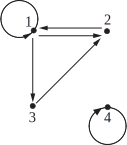
\includegraphics{figps-prev72digraph.eps}
\caption{Directed Graph for a Relation} \label{fig:dirgraph2}
\end{center}
\end{figure}

In a directed graph, the points are called the \textbf{vertices}.  So each element of  $A$  corresponds to a \textbf{vertex}.
\index{vertex}%
\index{directed graph!vertex}%
  The arrows, including the loops, are called the \textbf{directed edges}
\index{directed edge}%
\index{directed graph!directed edge}%
 of the directed graph.  We will make use of these directed graphs in the next section when we study equivalence relations.

\begin{prog}[\textbf{The Directed Graph of a Relation}]\label{prog:directedgraph} \hfill \\
Let $A = \{ 1, 2, 3, 4, 5, 6 \}$.  Draw a directed graph for the following two relations on the set $A$.  For each relation, it may be helpful to arrange the vertices of $A$ as shown in Figure~\ref{fig:dirgraph3}.
\[
R = \{ (x, y) \in A \times A \mid x \text{ divides } y \}, \qquad 
T = \{ (x, y) \in A \times A \mid x + y \text{ is even} \}.
\]
\begin{figure}[h]
\begin{center}
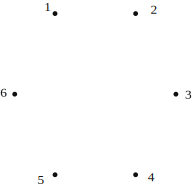
\includegraphics{figps-sec71-dirgraph.eps}
\caption{Vertices for $A$} \label{fig:dirgraph3}
\end{center}
\end{figure}
\end{prog}
\hbreak

\endinput


